\addcontentsline{toc}{part}{Appendices}

\newpage
\part*{Appendices}
\section{Appendix Section One}
\label{app:appendix-section-one}

%Example Table
\begin{table}[H]
\centering
\caption{\textit{Preliminary reactor specifications}}
\begin{tabular}{|c|c|c|c|c|c|}
\hline
\centering 
\textbf{Code}   & \textbf{Process Equipment} & \textbf{T (K)} & \textbf{P (bar)} & \textbf{Rating (kW)} & \textbf{Estimated Size (L)} \\
\hline
RX101& Packed Bed Reactor & 353.15 & 1.01325 & -16.31 & 1542.26\\
\hline
RX102 & CSTR & 271.15 & 1.01325 & -24.43 & 3303.29 \\
\hline 
RX103 & CSTR & 298.15 & 1.01325 & -5.53 & 1471.69 \\
\hline 
RX104 & Neutralisation Reactor & 298.15 & 1.01325 & -17.81 & 315.13 \\
\hline 
RX105 & Bubble Column Reactor & 293.15 & 1.01325 &-5.35 &  709.71\\
\hline
RX106 & CSTR & 303.15 & 1.01325 & -0.66 & 132.60 \\
\hline
RX107 & CSTR & 289.15 & 1.01325 & -33.51 & 65.50 \\
\hline
RX108 & Bubble Column Reactor & 353.15 & 1.01325 & -4.27 & 481.70 \\
\hline 
\end{tabular}
\centering
\label{table:reactor_specs}
\end{table}


%Example Figure
\begin{figure} [H]
     \centering
     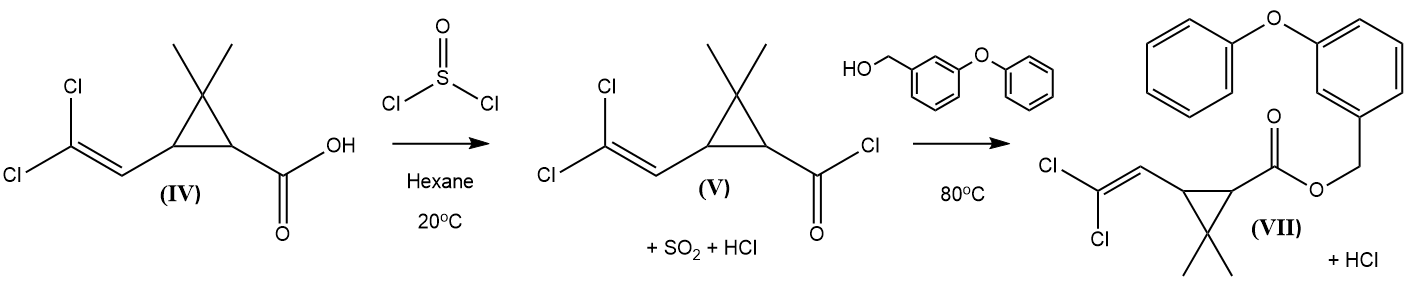
\includegraphics 
     [width=\linewidth]{figures/Permethrin.PNG}
     \caption{\textit{Permethrin reaction pathway adapted from UPL}}
     \label{fig:permethrin_process}
\end{figure}